\subsection{Begrænsninger}
\begin{frame}
	\frametitle{Begrænsninger - Analyse}
	Interviews
	\begin{itemize}
		\item Kontrol
	\end{itemize}
	Koncepter - State of the Art
	\begin{itemize}
		\item Flow
		\item Mixgar og specielt Rockbot
	\end{itemize}
\end{frame}

\begin{frame}
	\frametitle{Begrænsninger - Design}
	Black- og whitelisting
\end{frame}

\begin{frame}
	\frametitle{Begrænsninger - Design}
	Whitelisting
	
	\begin{equation}
		i \in A \textbf{ hvis og kun hvis } i \in W
	\end{equation}
	
	\begin{figure}
    \centering
    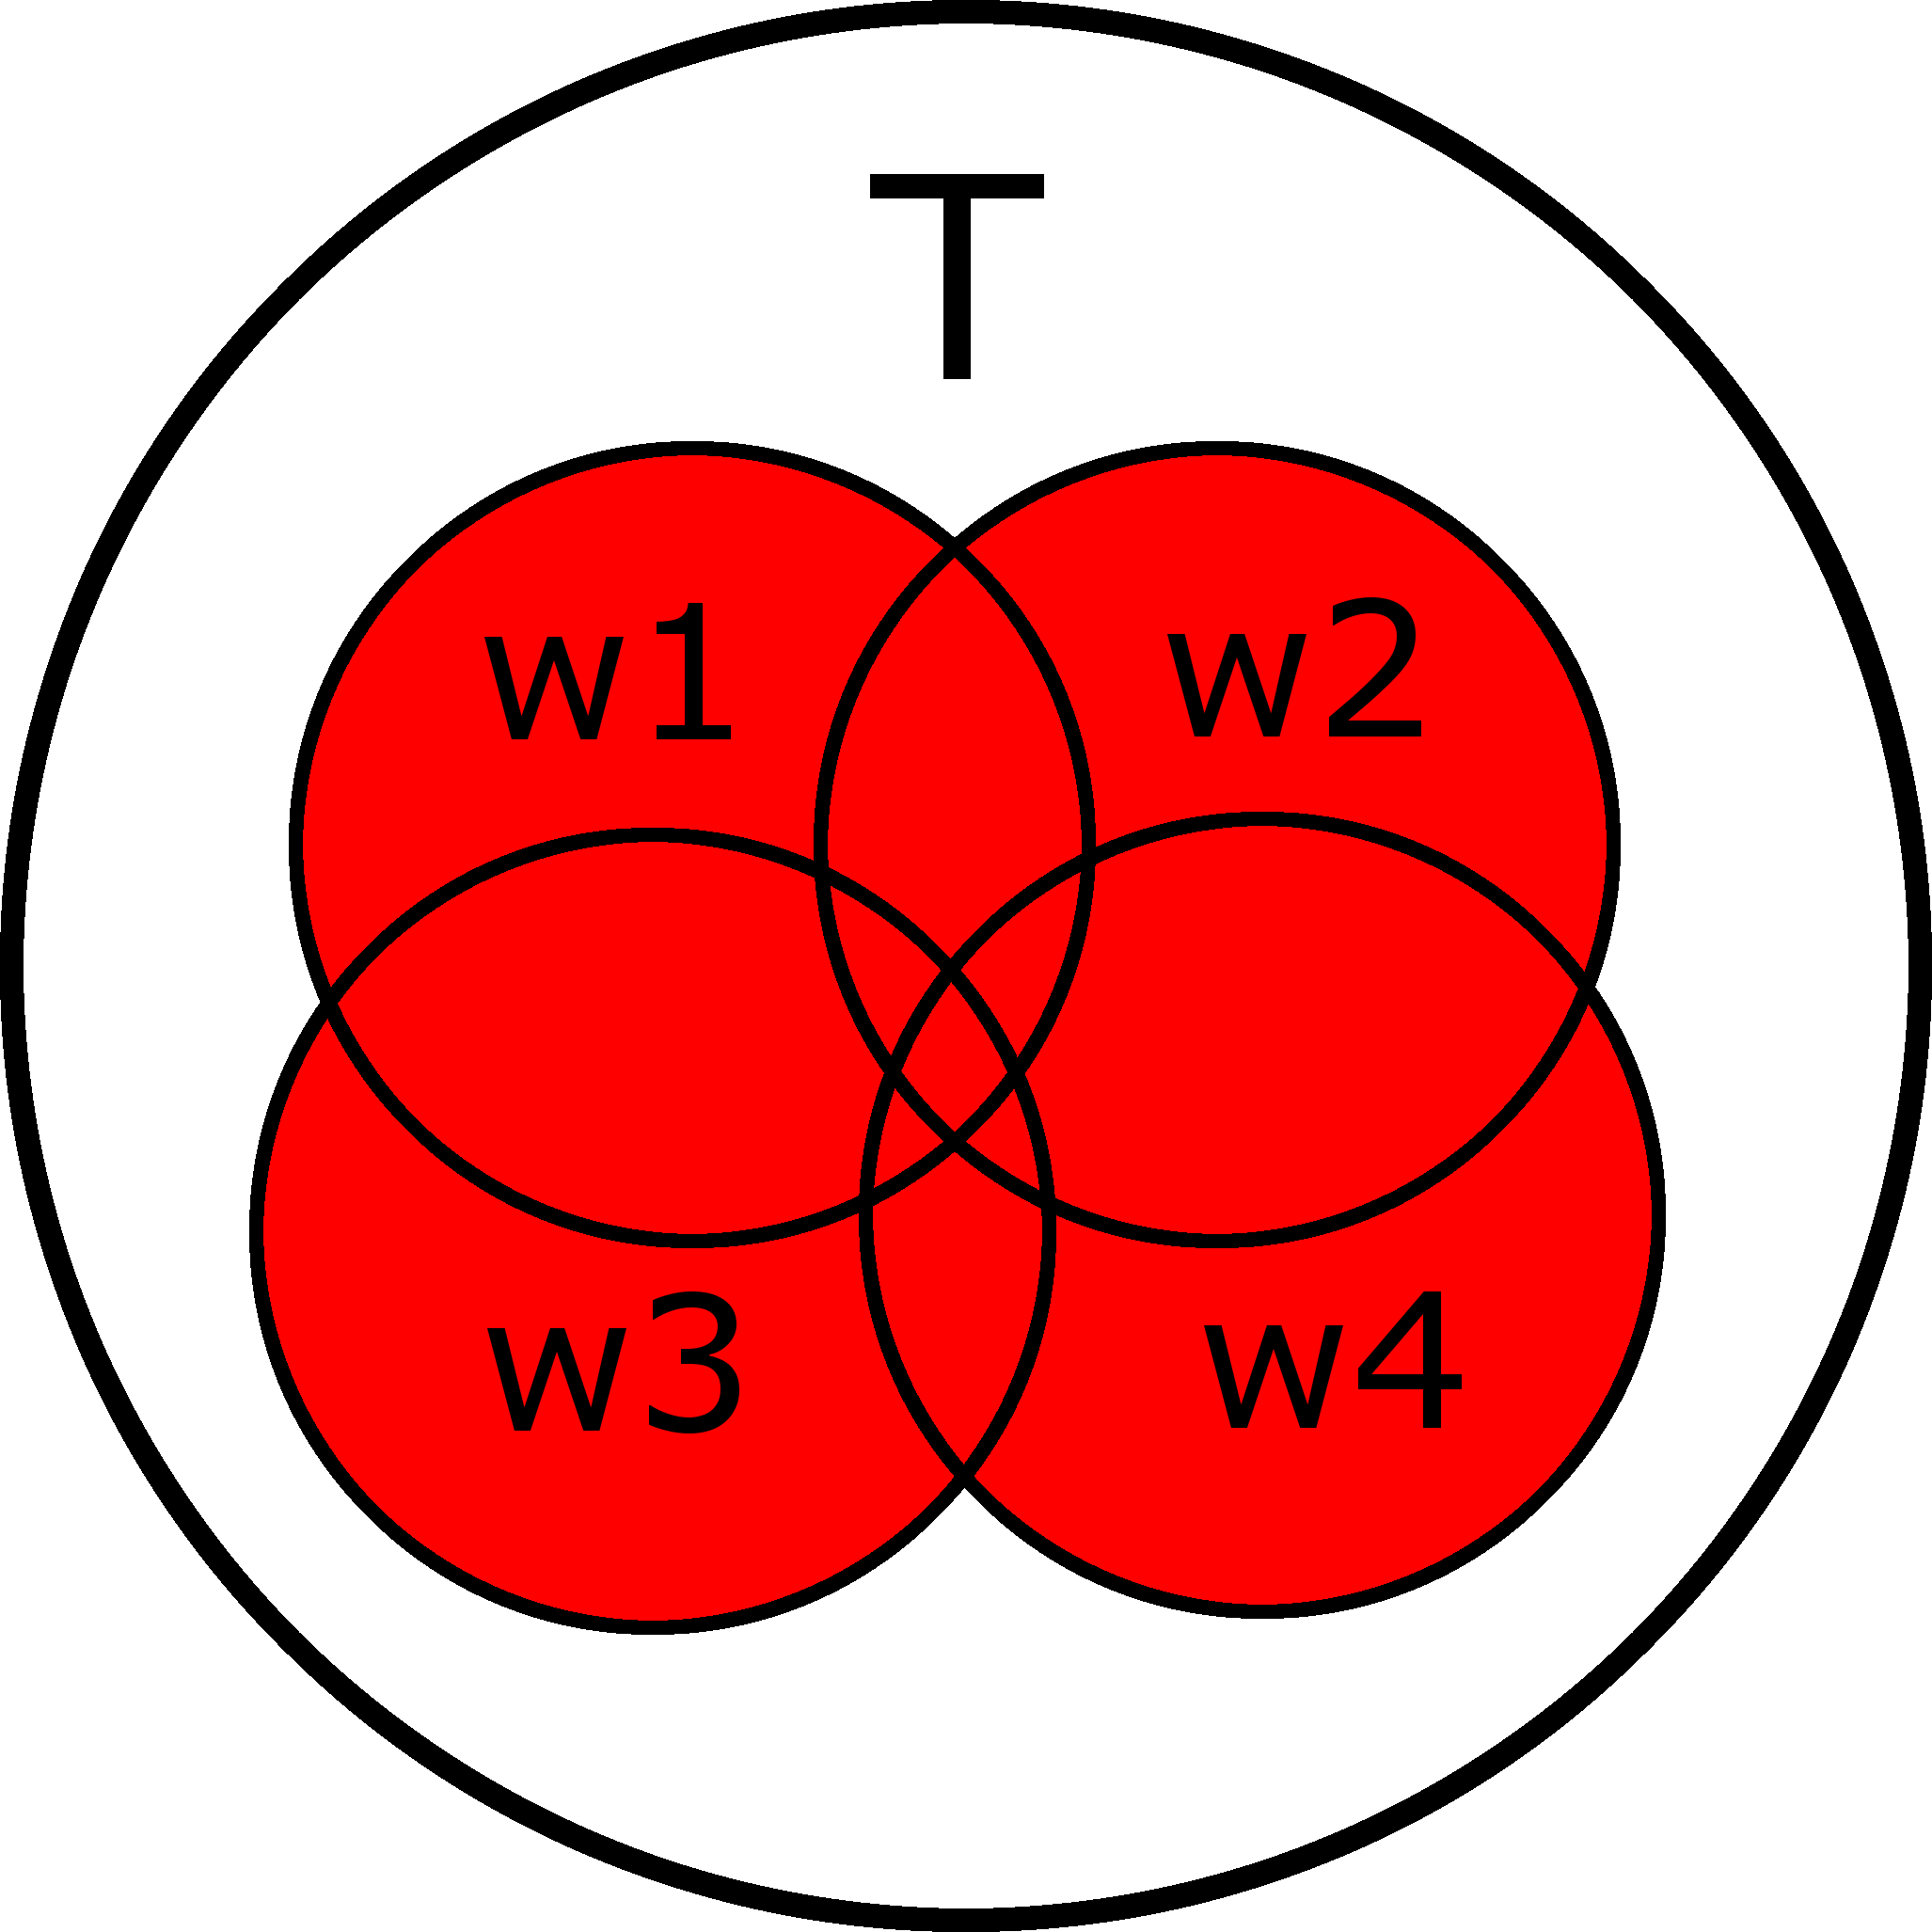
\includegraphics[width=100px]{slides/Jens/whitelist}
  \end{figure}
	
	\begin{equation}
		w_1 \vee w_2 \vee w_3 \vee \dots \vee w_n
	\end{equation}
\end{frame}

\begin{frame}
	\frametitle{Begrænsninger - Design}
	Blacklisting
	
	\begin{equation}
		i \in A \textbf{ hvis og kun hvis } i \notin B
	\end{equation}
	
	\begin{figure}
    \centering
    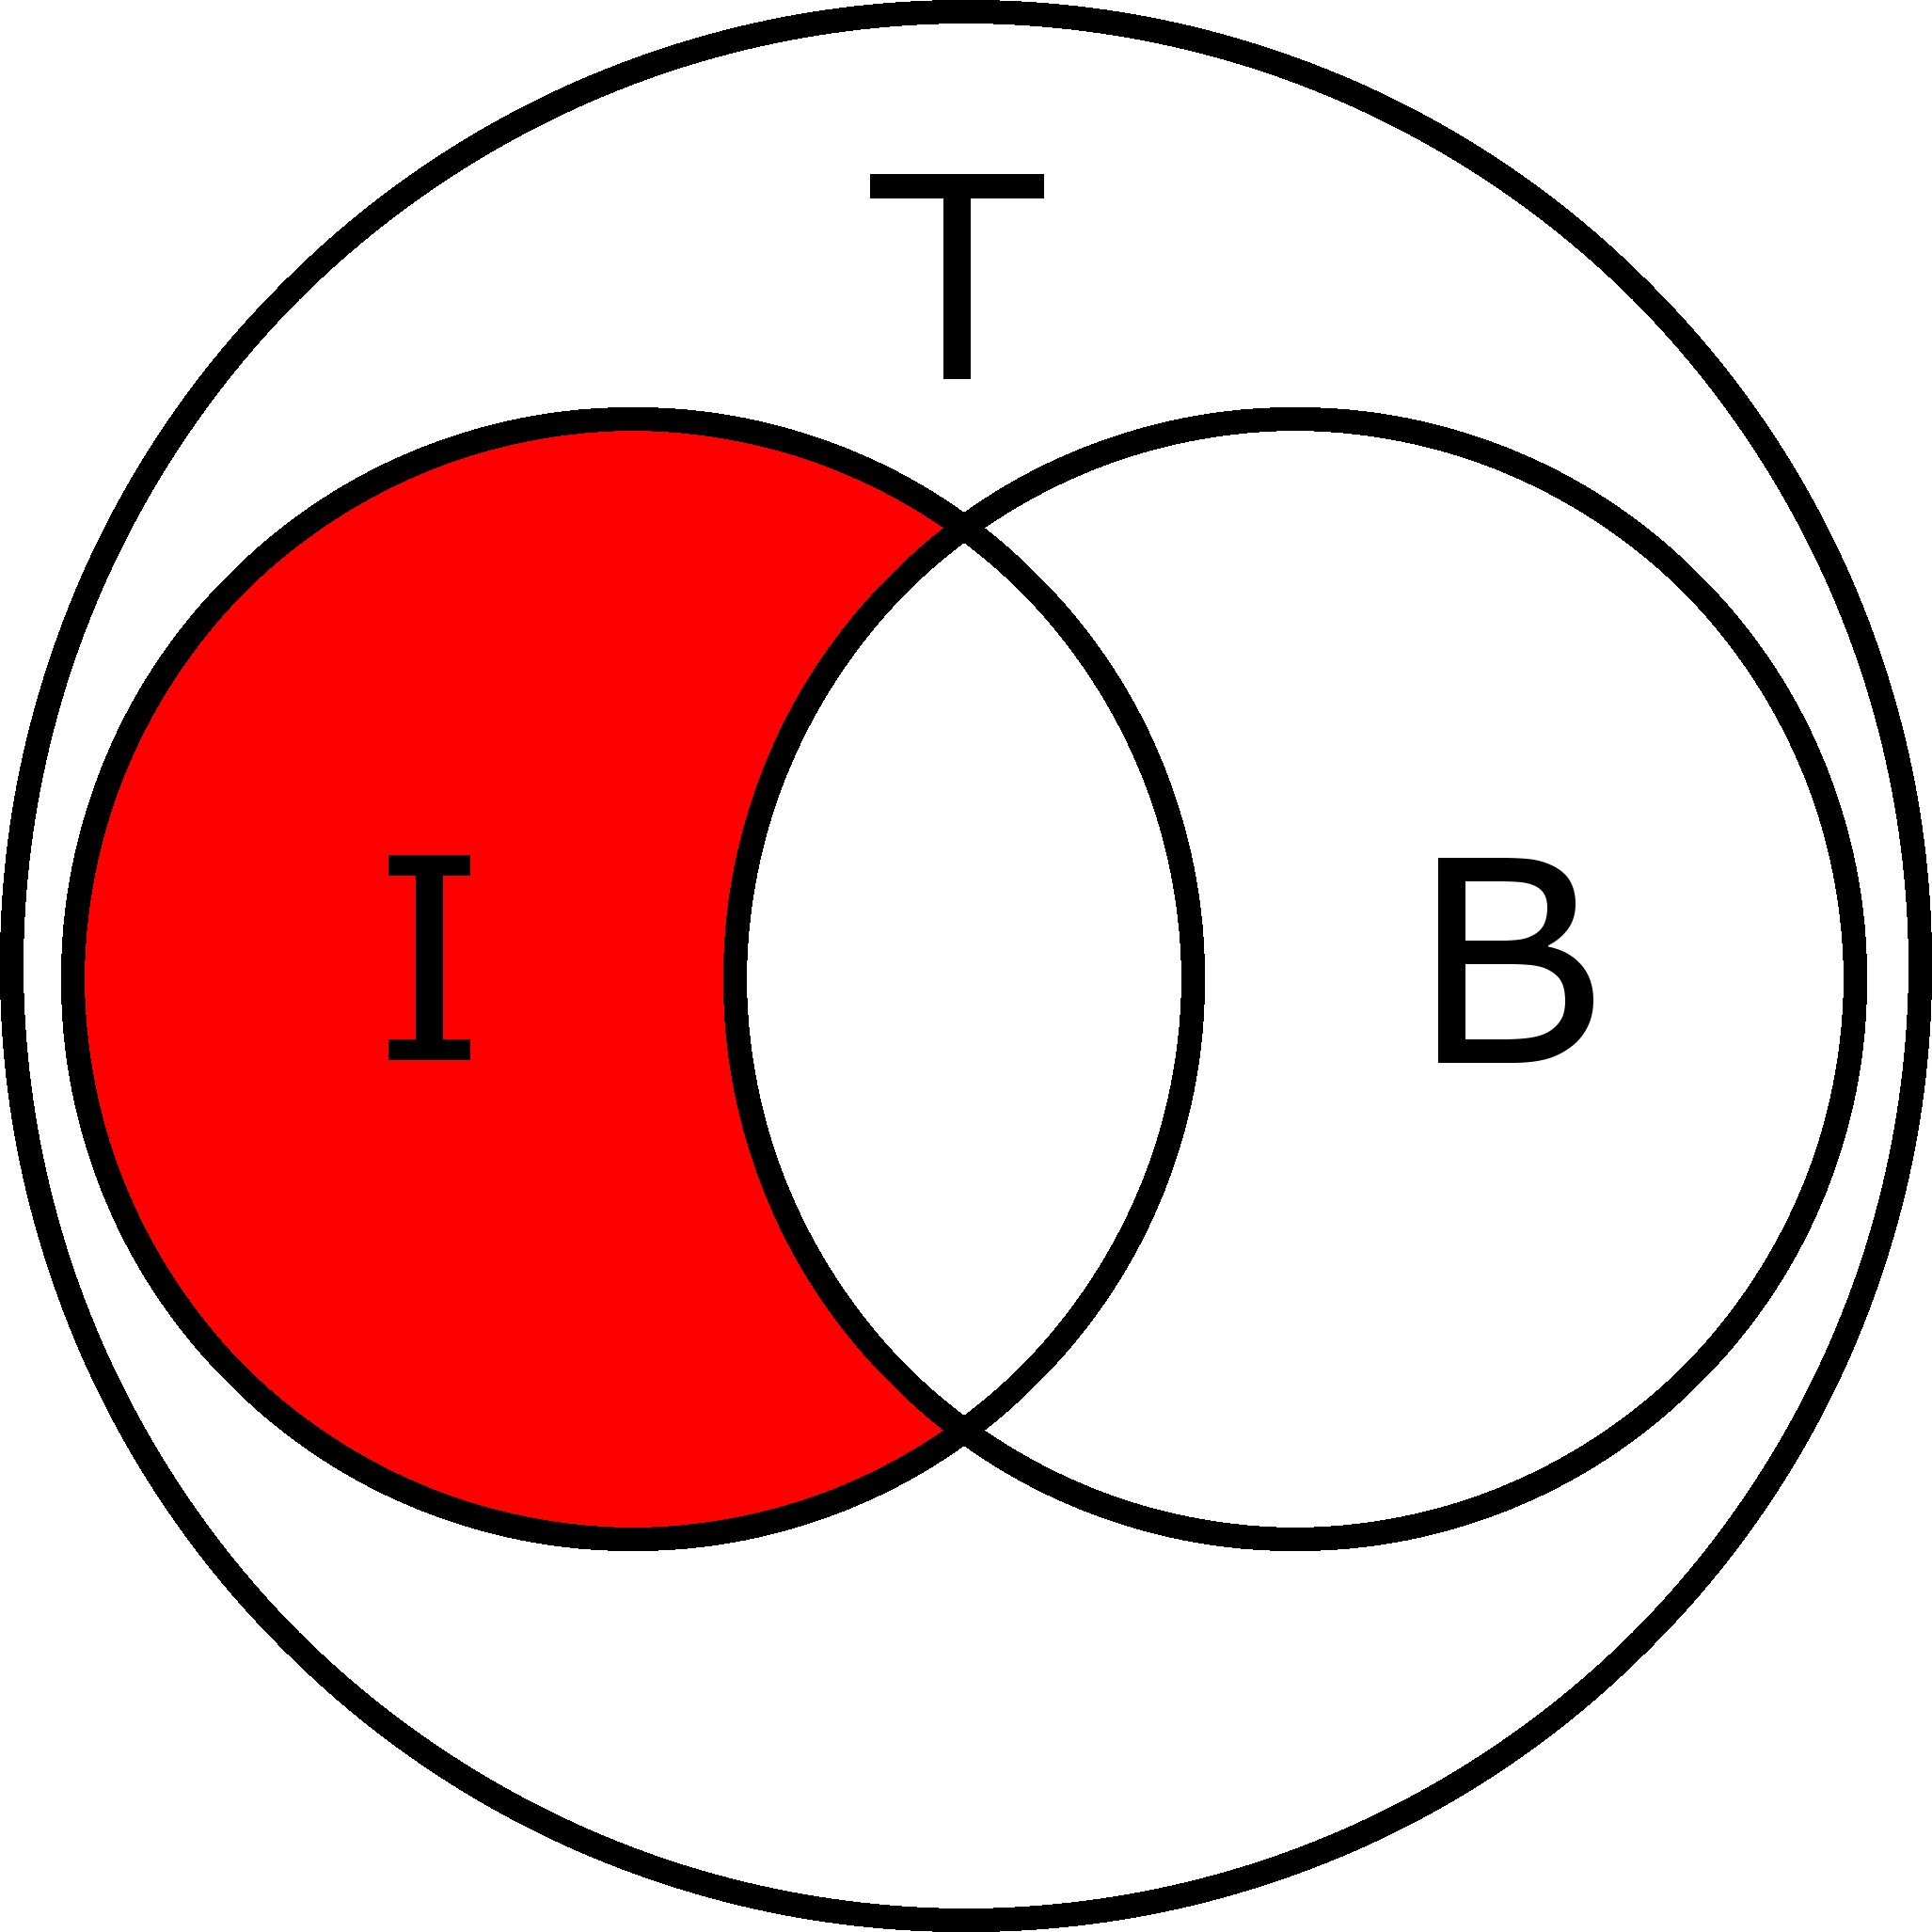
\includegraphics[width=100px]{slides/Jens/blacklist}
  \end{figure}
	
	\begin{equation}
		\neg(b_1 \vee b_2 \vee b_3 \vee \dots \vee b_n)
	\end{equation}
\end{frame}

\begin{frame}
	\frametitle{Begrænsninger - Design}
	Black- og whitelisting
	\begin{equation}
		(w_1 \vee w_2 \vee \dots \vee w_n) \wedge \neg(b_1 \vee b_2 \vee \dots \vee b_n)
	\end{equation}
	
	\begin{figure}
    \centering
    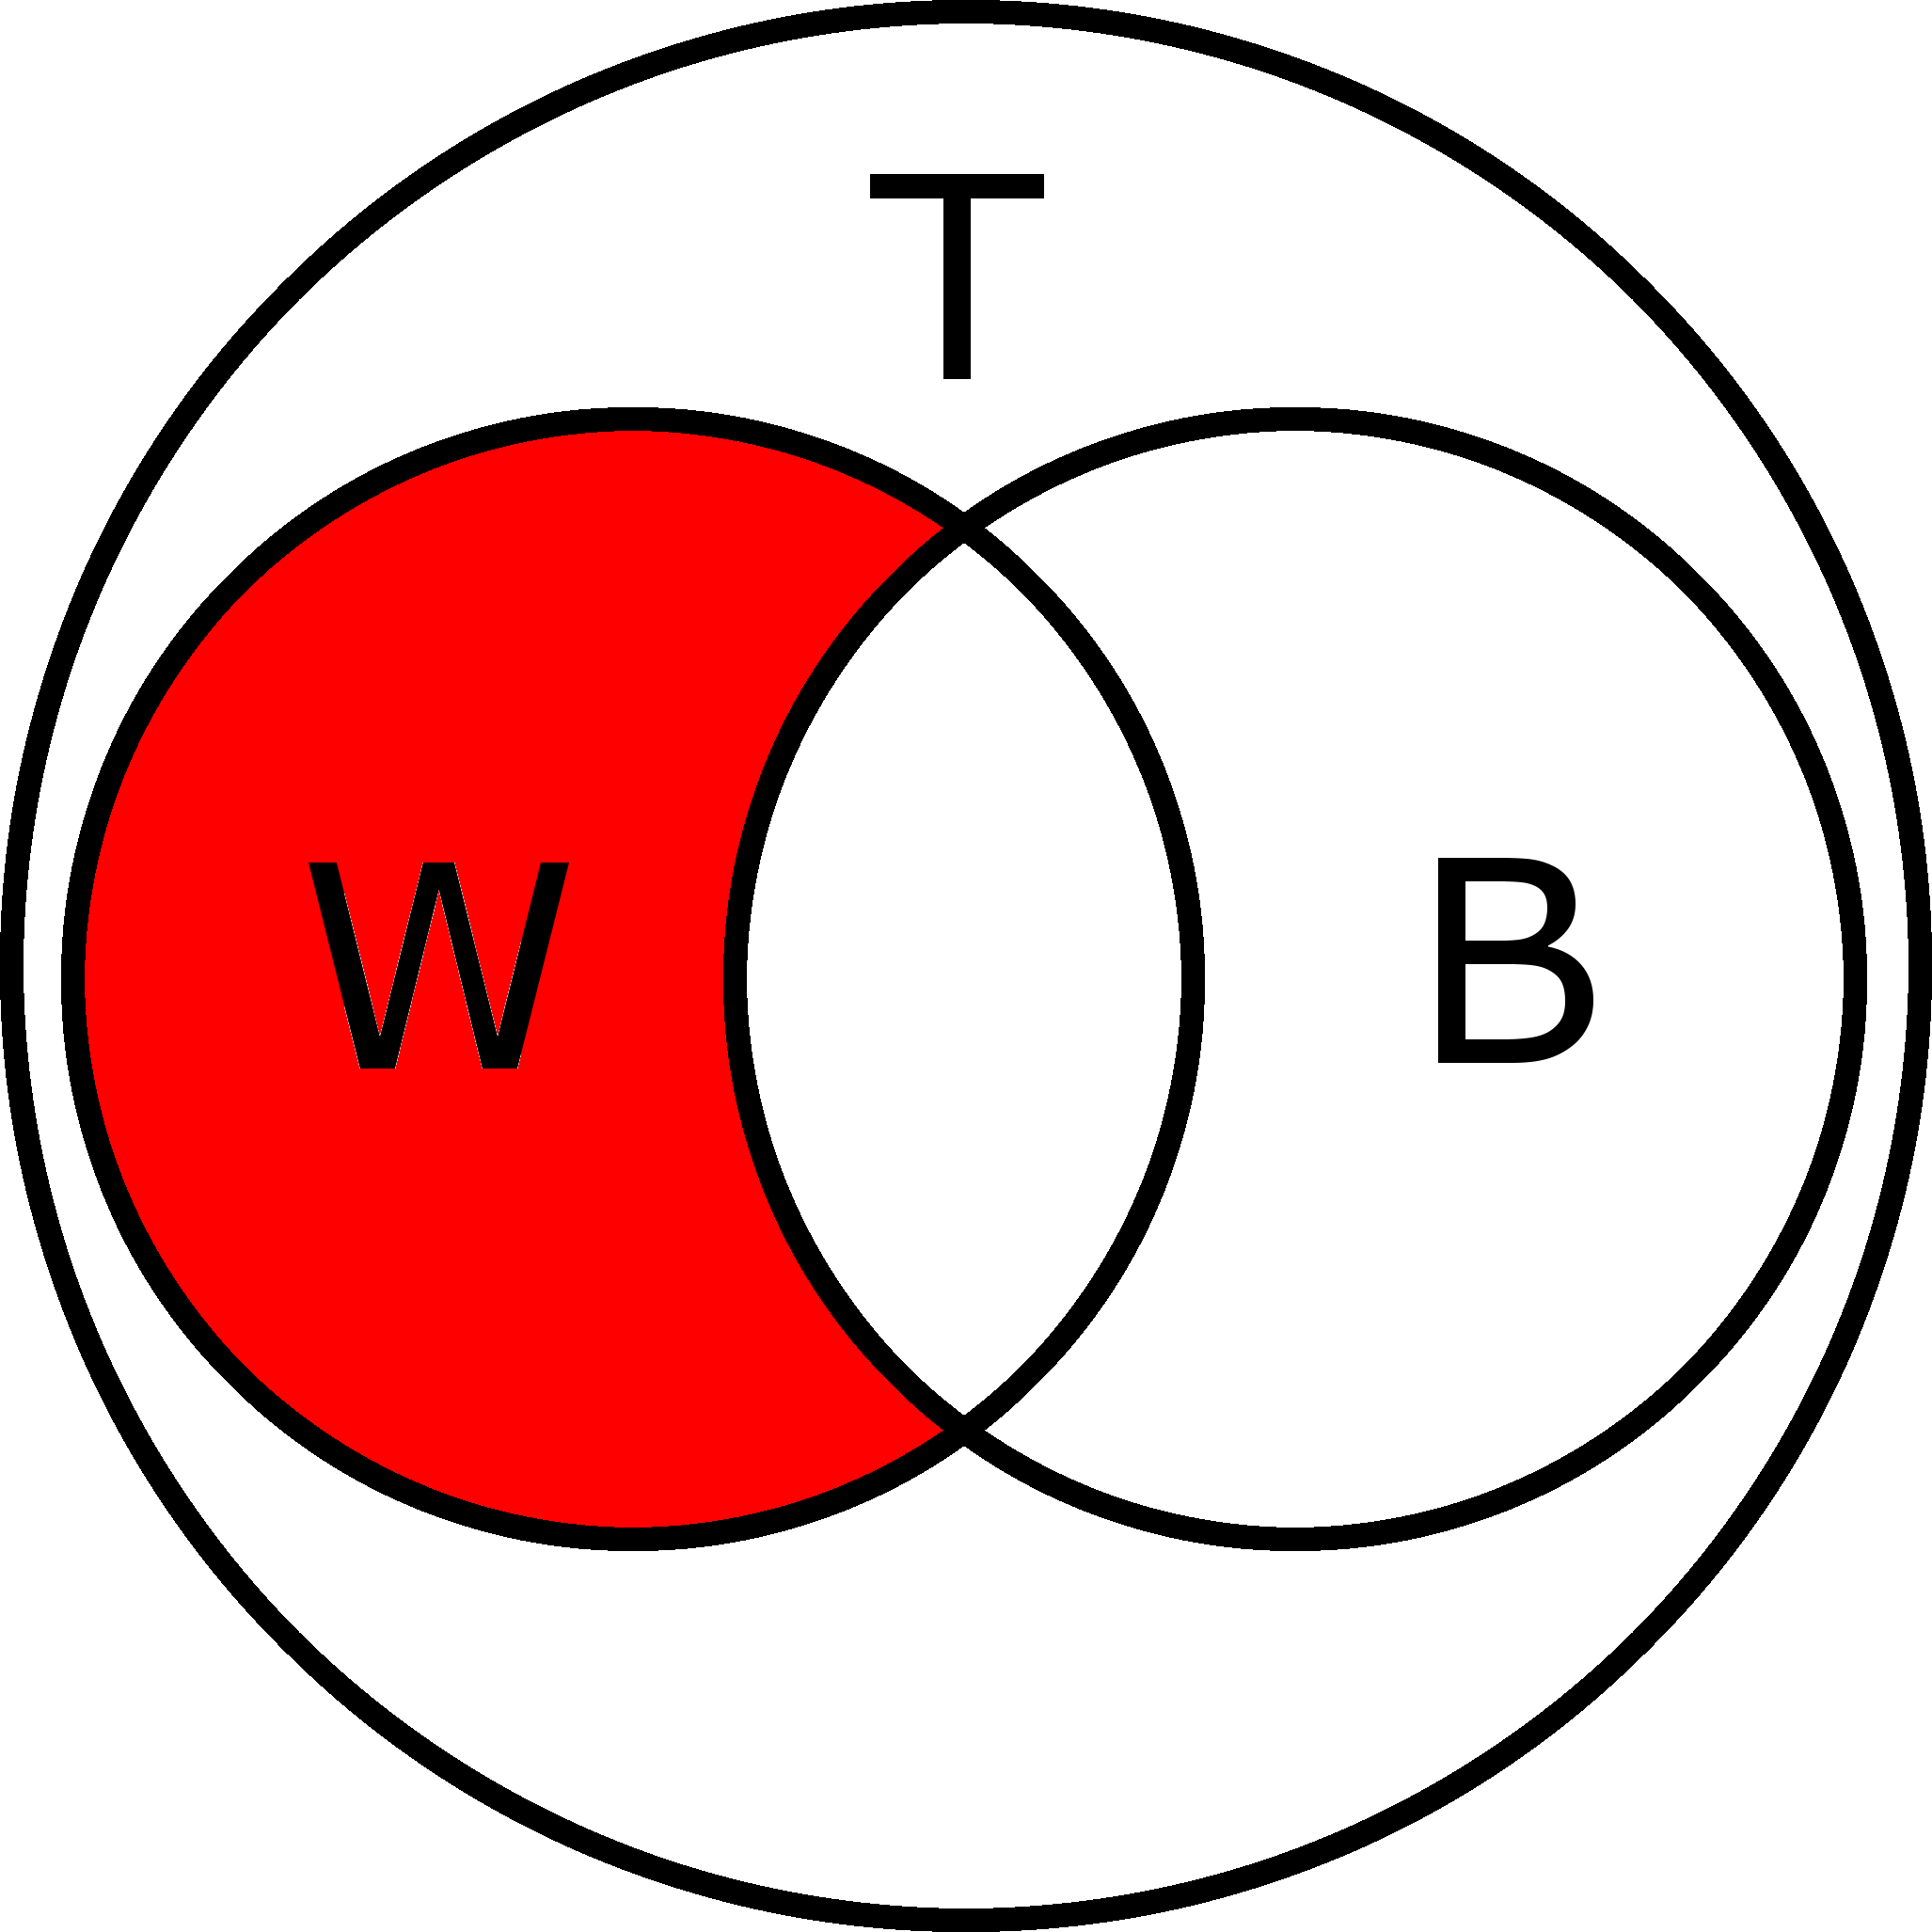
\includegraphics[width=100px]{slides/Jens/blackandwhitelist}
  \end{figure}
	
	%\begin{eqnarray}
	%\fontsize{8pt}{12}\selectfont
	%((w_{1.1} \wedge \dots \wedge w_{1.a}) \vee (w_{2.1} \wedge \dots \wedge w_{2.b}) \vee \dots \vee (w_{n.1} \wedge \dots \wedge w_{n.c})) \wedge \nonumber \\ \neg((b_{1.1} \wedge \dots \wedge b_{1.d}) \vee (b_{2.1} \wedge \dots \wedge b_{2.e}) \vee \dots \vee (b_{m.1} \wedge \dots \wedge b_{m.f}))
	%\end{eqnarray}
\end{frame}

\begin{frame}
\frametitle{Begrænsninger - Design}
\begin{algorithmic}[1]

	\Function{Search}{$query$, $restrictions$}
		\State{$results$ := $GetResults$($query$)}
		\ForAll{$track$ \textbf{in} $results$}
			\State{$track.IsAllowed$ := $Restrict$($track$,$restrictions$)}
		\EndFor
		\State{\Return{$results$}}
	\EndFunction{}
	
\end{algorithmic}
\end{frame}
		
\begin{frame}
\frametitle{Begrænsninger - Design}
\fontsize{9pt}{12}\selectfont
\begin{algorithmic}[1]
	\Function{Restrict}{$track$, $restrictions$}
		\State{$WhitelistExists$ := $false$}
		\State{$IsOnWhitelist$ := $false$}
		\State{$IsOnBlacklist$ := $false$}
		\ForAll{$restriction$ \textbf{in} $restrictions$}
			\If{$restriction$ \textbf{is} $whitelist$}
				\State{$WhitelistExists$ := $true$}
				\State{$IsOnWhitelist$ := $IsOnWhitelist$ $\vee$ $restriction$($track$)}
			\ElsIf{$restriction$ \textbf{is} $blacklist$}
				\State{$IsOnBlacklist$ := $IsOnBlacklist$ $\vee$ $restriction$($track$)}
			\EndIf{}
		\EndFor{}
		\State{\Return{($WhitelistExists$ $\to$ $IsOnWhitelist$) $\wedge$ $\neg IsOnBlacklist$}}
	\EndFunction{}
\end{algorithmic}
\end{frame}

\begin{frame}
	\frametitle{Begrænsninger - Implementation}
	    \centering
    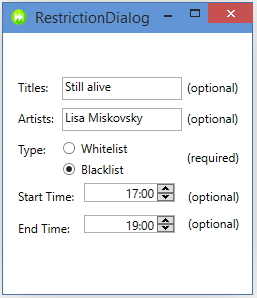
\includegraphics[width=100px]{slides/Jens/ServerInterfaceRestrictionDialog}
\end{frame}